\documentclass[a4paper,10pt,ngerman]{scrartcl}
\usepackage{babel}
\usepackage[T1]{fontenc}
\usepackage[utf8x]{inputenc}
\usepackage[a4paper,margin=2.5cm,footskip=0.5cm]{geometry}

% todo: check TeilnahmeId
\newcommand{\Aufgabe}{Aufgabe 3: Eisbudendilemma}
\newcommand{\TeilnahmeId}{56860}
\newcommand{\Name}{Christopher Besch}


% header and footer
\usepackage{scrlayer-scrpage, lastpage}
\setkomafont{pageheadfoot}{\large\textrm}
\lohead{\Aufgabe}
\rohead{Teilnahme-ID: \TeilnahmeId}
\cfoot*{\thepage{}/\pageref{LastPage}}

% title position
\usepackage{titling}
\setlength{\droptitle}{-1.0cm}

% for math commands and symbols
\usepackage{amsmath}
\usepackage{amssymb}

% for images
\usepackage{graphicx}
\graphicspath{{images/}}
\usepackage{subcaption}

% for tables
\usepackage{tabularx}

% for algorithms
\usepackage{algpseudocode}

% for source code
\usepackage{listings}
\usepackage{color}
\definecolor{mygreen}{rgb}{0,0.6,0}
\definecolor{mygray}{rgb}{0.5,0.5,0.5}
\definecolor{mymauve}{rgb}{0.58,0,0.82}
\lstset{
  keywordstyle=\color{blue},commentstyle=\color{mygreen},
  stringstyle=\color{mymauve},rulecolor=\color{black},
  basicstyle=\footnotesize\ttfamily,numberstyle=\tiny\color{mygray},
  captionpos=b, % sets the caption-position to bottom
  keepspaces=true, % keeps spaces in text
  numbers=left, numbersep=5pt, showspaces=false,showstringspaces=true,
  showtabs=false, stepnumber=2, tabsize=2, title=\lstname
}
\lstdefinelanguage{JavaScript}{ % JavaScript is the only non-predefined language
  keywords={break, case, catch, continue, debugger, default, delete, do, else, finally, for, function, if, in, instanceof, new, return, switch, this, throw, try, typeof, var, void, while, with},
  morecomment=[l]{//},
  morecomment=[s]{/*}{*/},
  morestring=[b]',
  morestring=[b]",
  sensitive=true
}

% these packages must be loaded last
\usepackage{hyperref}
\usepackage{cleveref}

% c++ source code setup
\lstset{
    language=C++,
    basicstyle=\small\sffamily,
    numbers=left,
    numberstyle=\tiny,
    frame=tb,
    tabsize=4,
    columns=fixed,
    showstringspaces=false,
    showtabs=false,
    keepspaces,
    commentstyle=\color{red},
    keywordstyle=\color{blue}
}

% title
\title{\textbf{\Huge\Aufgabe}}
\author{\LARGE Teilnahme-ID: \LARGE \TeilnahmeId \\\\
	    \LARGE Bearbeiter/-in dieser Aufgabe: \\ 
	    \LARGE \Name\\\\}
\date{\LARGE\today}

\begin{document}

\maketitle
\tableofcontents

\vspace{0.5cm}

\section{Ein Wort über die Graphiken}
Alle in dieser Dokumentation verwendeten Darstellungen verwenden einheitliche Symbole:
\begin{itemize}
    \item Der See ist als schwarzer Kreis dargestellt.
    \item Die Häuser sind verschieden gefärbte Rechtecke, deren Adresse außerhalb des Kreises stehen:
          \begin{itemize}
              \item Rot: Das Haus stimmt gegen eine Verlegung der Eisdielen.
              \item Grün: Es stimmt für eine Verlegung.
              \item Andere Farben werden verwendet, um bestimmte Häuser herauszuheben.
                    Die jeweiligen Bedeutungen werden darstellungsspezifisch angegeben.
          \end{itemize}
    \item Die Adressen sind aufsteigend im Uhrzeigersinn angeordnet.
          Adresse $0$, die Dorfkirche befindet sich oben.
    \item Blaue Kreuze stellen die Positionen des Test-Arrangements dar und
    \item blaue Kreise die des Check-Arrangements.
          In beiden Fällen stehen die Adressen innerhalb des Kreises.
\end{itemize}

\section{Lösungsidee}
% Die Idee der Lösung sollte hieraus vollkommen ersichtlich werden, ohne dass auf die eigentliche Implementierung Bezug genommen wird.
Das Ziel ist es, ein Arrangement bestehend aus drei Positionen für Eisdielen zu generieren, das in einer Abstimmung durch kein anderes Arrangement abgelöst werden kann.
Diese Arrangements werden stabil genannt.
Hierzu darf die Eisbudendistanz, die Strecke zwischen einem beliebigen Haus und der nächsten Eisbude, von nicht mehr als der Hälfte der Hauser durch ein anderes Arrangement verkürzt werden.
Wäre dies der Fall, würde die Ablösung mehr Ja- als Nein-Stimmen erhalten.
Hieraus geht hervor, dass für eine optimale Lösung alle möglichen Arrangements (Diese werden Test-Arrangement genannt.) auf Stabilität überprüft werden müssen.
Um die Stabilität zu bestimmen, muss das Test-Arrangement mit allen möglichen anderen Arrangements (Check-Arrangement genannt) verglichen werden.
Wenn auch nur ein einziges Check-Arrangement gefunden wird, das mehr Ja- als Nein-Stimmen erhält, ist das getestete Test-Arrangement instabil.
Es lässt sich leicht erkennen, dass dieser Algorithmus, der Durchgang aller möglichen Test-Arrangements, mit einer Laufzeit von $O(n^6)$ nicht verwendbar ist.

\medskip
Als Versuch der Optimierung werden bevor sie getestet werden alle Arrangement sortiert.
Hierzu wird für jedes mögliche Arrangement ein Score berechnet.
Dieser entspricht der durchschnittlichen Eisbudendistanz aller Häuser.
Nun stellt sich heraus, dass stabile Arrangements einen der niedrigsten Scores aller Arrangements aufweisen.
Dies lässt sich damit erklären, dass je kleiner die Eisbudendistanz eines Hauses in einem Test-Arrangement ist, desto weniger Check-Arrangement existieren, die eine noch geringere Eisbudendistanz für das Haus generieren.
Wenn die Eisbudendistanz beispielsweise $0$ beträgt, existiert kein einziges Check-Arrangement, dem dieses Haus eine Ja-Stimme geben würde, da eine geringere Eisbudendistanz nicht möglich ist und ein Haus bei gleichbleibender Eisbudendistanz immer gegen einen Wechsel stimmt.
Dies ist in \autoref{fig:01_hapy_house} gezeigt.
\begin{figure}[ht]
    \centering
    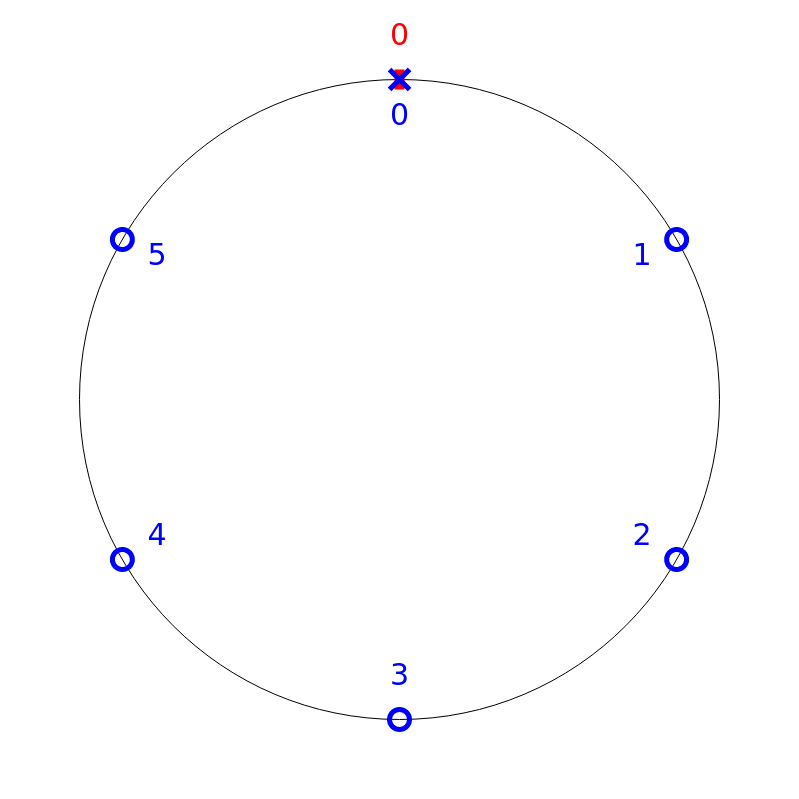
\includegraphics[width=0.4\linewidth]{01_happy_house.png}
    \caption{Das einzige Haus ist zufrieden mit der einzigen Eisdiele und lehnt jegliche Veränderung ab. Die Eisbudendistanz beträgt $0$.}
    \label{fig:01_hapy_house}
\end{figure}
Wenn die Eisbudendistanz den maximalen Wert, dem halben Umfang des Sees, entspricht, stimmt es für alle Check-Arrangements (\autoref{fig:02_unhappy_house}), abgesehen von denen, die die Eisbudendistanz nicht verändern (\autoref{fig:03_slightly_happy_house}).
\begin{figure}[ht]
    \centering
    \caption{Unzufriedene Häuser}
    \begin{subfigure}[t]{0.4\linewidth}
        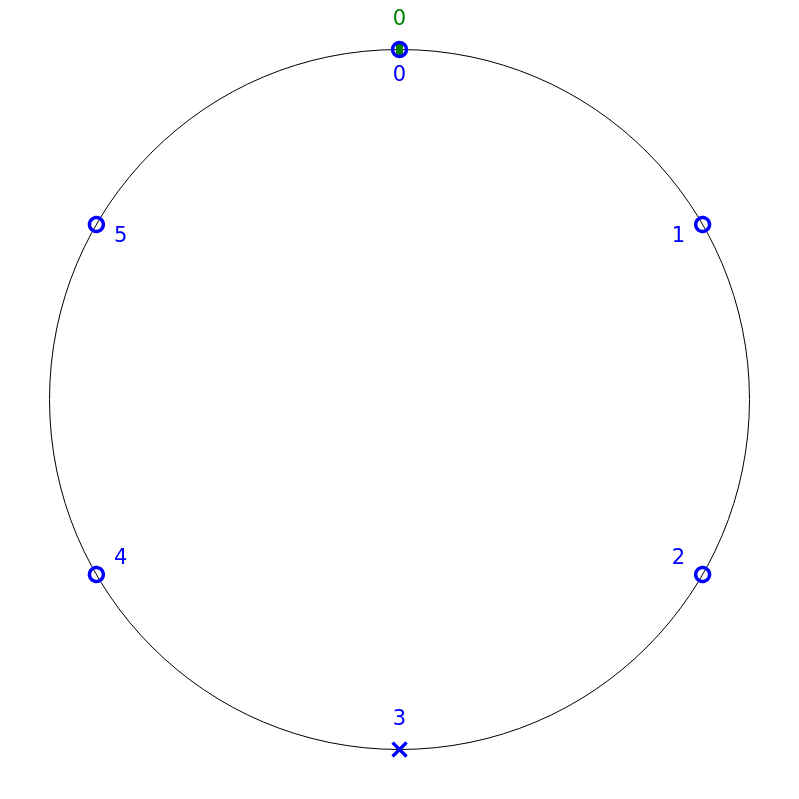
\includegraphics[width=\linewidth]{02_unhappy_house.png}
        \caption{Das Haus ist maximal unzufrieden, weshalb es für fast jede Verlegung stimmt. Jeder Kreis repräsentiert eine anderes Check-Arrangement, die alle von dem Haus angenommen werden.}
        \label{fig:02_unhappy_house}
    \end{subfigure}
    \begin{subfigure}[t]{0.4\linewidth}
        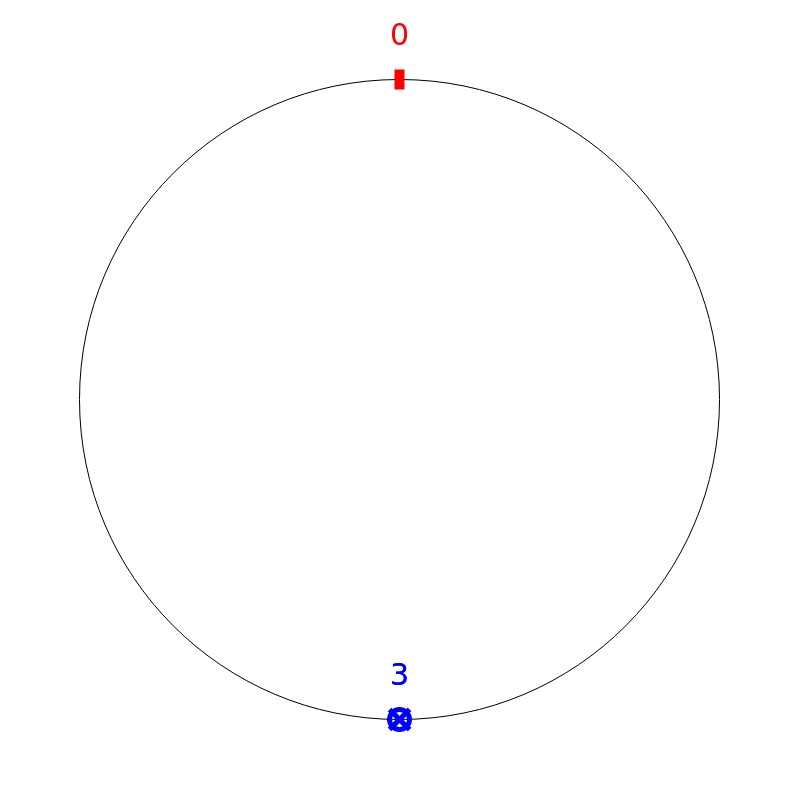
\includegraphics[width=\linewidth]{03_slightly_happy_house.png}
        \caption{Dies ist der einzige Fall, in dem das Haus trotz seiner extremen Unzufriedenheit gegen eine Verlegung stimmt.}
        \label{fig:03_slightly_happy_house}
    \end{subfigure}
\end{figure}
Die durchschnittliche Eisbudendistanz lässt sich dementsprechend als \glqq Zufriedenheitsgrad\grqq{} des Dorfes interpretieren.
Je höher er ist, desto unwahrscheinlicher wird eine Verlegung durchgesetzt.

Allerdings muss dieser Wert nicht zwangsweise mit der Stabilität eines Arrangements übereinstimmen, was beispielsweise in \autoref{fig:04_borken_example} gezeigt wird.
\begin{figure}[ht]
    \centering
    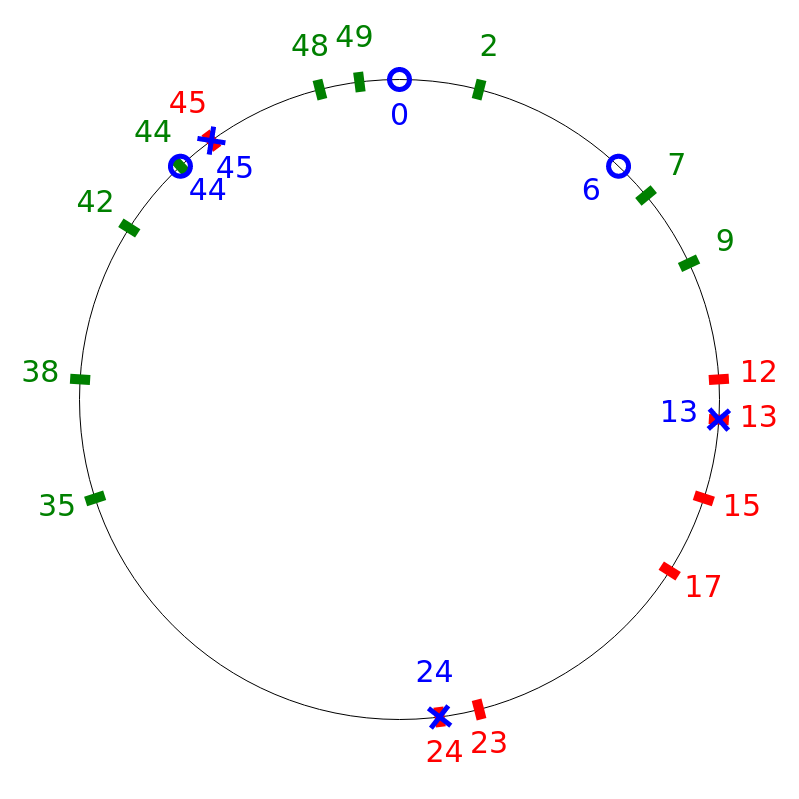
\includegraphics[width=0.4\linewidth]{04_broken_example.png}
    \caption{Trotz der für dieses Beispiel, \textit{eisbuden3.txt}, minimalen durchschnittlichen Eisbudendistanz von $3,3125$ stimmen mehr Häuser für eine Verlegung.}
    \label{fig:04_borken_example}
\end{figure}
Hieraus geht hervor, dass die durchschnittliche Eisbudendistanz nur eine Näherungslösung liefert.
Trotzdem kann sie zur Generierung eines Satzes an Test-Arrangements verwendet werden, die anschließend von dem bereits genannten Algorithmus auf Stabilität überprüft werden.

\medskip
Um die Stabilität eines Test-Arrangements zu berechnen, müssen alle möglichen Check-Arrangements durchgegangen werden.
Es wird nur eine einziges Check-Arrangement gesucht, das das Test-Arrangement schlagen kann.
Daher können zwei Optimierungen getroffen werden:
\begin{enumerate}
    \item Eisdielen sollten nicht übereinander liegen, da bei der Aufsplittung zweier aufeinanderliegender Eisdielen die Eisbudendistanz keines Häuses vergrößert wird.
    \item Alle Dopplungen sind unnötig, da die Reihenfolge der Eisdielen für die Stimmen der Häuser irrelevant sind.
\end{enumerate}
Deshalb darf die Bedingung gelten, dass die Adresse der zweiten Eisdiele größer als die der ersten und kleiner als die der dritten ist.
Hieraus folgt, dass der See in drei Sektoren unterteilt ist (\autoref{fig:05_sectors}).
\begin{figure}[ht]
    \centering
    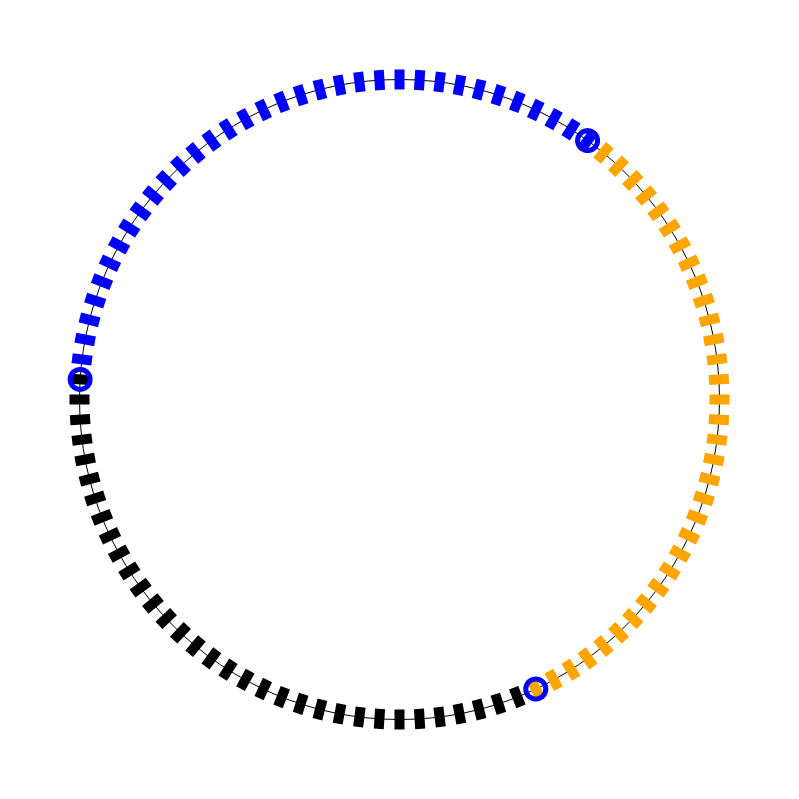
\includegraphics[width=0.4\linewidth]{05_sectors.png}
    \caption{Einteilung in Sektoren}
    \label{fig:05_sectors}
\end{figure}

Um nun alle Position durchzugehen, können zuerst zwei Positionen für die ersten beiden Eisdielen festgesetzt werden (Die verschiedenen Optionen für diese müssen in einem übergeordneten Schritte durchgegangen werden) und daraufhin alle möglichen Positionen für die dritte Eisdiele verwendet werden, die die genannten Bedingungen erfüllt.
Somit ist die Größe und Position des ersten Sektor bei vielen Durchläufen gleich.

Nun zeigt sich, dass die Stimme der Häuser innerhalb eines Sektors ausschließlich durch die Größe und Position des Sektors und die in dem Sektor befindlichen Eisdielen des Test-Arrangements determiniert sind.
Dies lässt sich dadurch begründen, dass die Eisdielendistanzen dieser Häuser nur dann nicht verkürzt werden, wenn sich eine Eisdiele des Test-Arrangements in dem Sektor befindet.
Alle Test-Eisdielen außerhalb des Sektors sind von den Häusern immer weiter entfernt als die Ränder des Sektors, weshalb sich die Eisbudendistanz ohne Test-Eisdielen innerhalb des Sektors nicht verkürzt wird.

\medskip
In der Implementation wird auf viele Optimierungen eingegangen





















\section{Umsetzung}
% Hier wird kurz erläutert, wie die Lösungsidee im Programm tatsächlich umgesetzt wurde. Hier können auch Implementierungsdetails erwähnt werden.
Die Lösungsidee wird in C++ implementiert.

\paragraph{Einlese der Eingabedatei}
Als erster Schritt wird in der Funktion \textbf{read\_file} die Eingabedatei gelesen.
Hierbei wird überprüft, ob die Eingabedatei dem gegebenen Format entspricht, wenn nicht wird das Programm abgebrochen.
Hierzu wird ein Makro \textbf{raise\_error()} verwendet, dass die Ausführung des Programmes abbricht und eine möglichst informative Fehlermeldung zurückgibt.
Dieses Makro wird ebenfalls für alle Methoden aller Klassen verwendet, um z.b. Segmentation Faults zu verhindern.

Es wird die Menge der Adressen aller Häuser in einem std::vector<int> und der Umfang des Sees in einem int gespeichert.


\section{Beispiele}
% Genügend Beispiele einbinden! Die Beispiele von der BwInf-Webseite sollten hier diskutiert werden, aber auch eigene Beispiele sind sehr gut – besonders wenn sie Spezialfälle abdecken. Aber bitte nicht 30 Seiten Programmausgabe hier einfügen!
Nun wird das Programm mit allen Beispieldateien ausgeführt.

\paragraph{eisbuden1.txt}
Mit der Eingabe

20 7

0 2 3 8 12 14 15

gibt das Programm aus, dass es keine stabilen Positionen gibt.

\paragraph{eisbuden2.txt}
Mit der Eingabe

50 15

3 6 7 9 24 27 36 37 38 39 40 45 46 48 49

gibt das Programm die Menge an stabilen Positionen aus:

45

\paragraph{eisbuden3.txt}
Mit der Eingabe

50 16

2 7 9 12 13 15 17 23 24 35 38 42 44 45 48 49

gibt das Programm die Menge an stabilen Positionen aus:

2, 3, 4, 5, 6 und 7

\paragraph{eisbuden4.txt}
Mit der Eingabe

100 19

6 12 23 25 26 28 31 34 36 40 41 52 66 67 71 75 80 91 92

gibt das Programm die Menge an stabilen Positionen aus:

34

\paragraph{eisbuden5.txt}
Mit der Eingabe

247 24

2 5 37 43 72 74 83 87 93 97 101 110 121 124 126 136 150 161 185 200 201 230 234 241

gibt das Programm die Menge an stabilen Positionen aus:

93, 94, 95, 96 und 97

\paragraph{eisbuden6.txt}
Mit der Eingabe

437 36

4 12 17 23 58 61 67 76 93 103 145 154 166 170 192 194 209 213 221 225 239 250 281 299 312 323 337 353 383 385 388 395 405 407 412 429

gibt das Programm aus, dass es keine stabilen Positionen gibt.

\paragraph{eisbuden7.txt}

\subsection{Eigene Beispiele}

\paragraph{myeisbuden0.txt}
Mit der Eingabe

12 4

0 3 6 9

gibt das Programm die Menge an stabilen Positionen aus:

0, 1, 2, 3, 4, 5, 6, 7, 8, 9, 10 und 11

Dies ergibt Sinn, da die Häuser gleichmäßig verteilt sind, womit nie eine Mehrheit gegen jegliche Positionen gefunden werden kann.

\paragraph{myeisbuden0.txt}
Mit der Eingabe

10 0


0, 1, 2, 3, 4, 5, 6, 7, 8 und 9

Dies ergibt Sinn, da keine Häuser vorhanden sind, die für eine Umlegung stimmen könnten.

\section{Quellcode}
% Unwichtige Teile des Programms sollen hier nicht abgedruckt werden. Dieser Teil sollte nicht mehr als 2–3 Seiten umfassen, maximal 10.
Dies sind die wichtigsten Funktionen:
\begin{lstlisting}
int get_distance(int circumference, int place_a, int place_b)
{
    int direct_distance = std::abs(place_a - place_b);
    // take shortest way, direct or the othe rdirection
    return std::min(direct_distance, circumference - direct_distance);
}

bool vote(int circumference, int house_place, int old_place, int new_place)
{
    // is new place better?
    if (get_distance(circumference, house_place, new_place) <
    get_distance(circumference, house_place, old_place))
        return true;
    return false;
}

bool is_stable(int circumference, std::vector<int> &houses, int test_place)
{
    // would any other place win an election against test_place?
    for (int other_place = 0; other_place < circumference; other_place++)
    {
        int trues = 0;
        for (int house : houses)
            if (vote(circumference, house, test_place, other_place))
                trues++;

        if (trues > houses.size() - trues)
            return false;
    }
    return true;
}

std::vector<int> get_stabel_places(int circumference, std::vector<int> &houses)
{
    // go thorugh all possible places
    std::vector<int> result;
    for (int test_place = 0; test_place < circumference; test_place++)
        if (is_stable(circumference, houses, test_place))
            result.push_back(test_place);
    return result;
}
\end{lstlisting}

\end{document}
